% Drawing 67/03-5 -- folder 67, batch 03, archive page 59 (PDF page 60).
% Transcription: dans la marge gauche, en regard du premier « Lemme 3 » barré, deux croquis. En haut, deux segments presque horizontaux l'un sous l'autre, chacun portant un point marqué vers son milieu et terminé à droite par un point noté « $1$ », hachurés l'un au-dessus, l'autre au-dessous (deux demi-plans), et une flèche verticale du premier au second. En bas, un demi-disque dont le diamètre porte un point marqué, d'où part un arc ondulé qui rejoint le demi-cercle.
% Kind: two sketches: two hatched half-planes glued along their edges; half-disc cut by an arc. Method 2 (schematic redraw from the facsimile). Status: ok.
% Notes: Top: the two edges, each drawn between its end points with the marked point computed on it; hatching above the upper edge and below the lower one (five oblique strokes each, as on the page); the end points and the two labels 1; the vertical arrow from the upper to the lower edge. Bottom: the diameter, the half-circle through its two ends, the heavy point on the diameter and the wavy arc from it to a computed point of the half-circle; a small hook under the point. Left out: the three long oblique strokes that strike the first « Lemme 3 » and cross the upper sketch; the words of the text at the right. Redrawn 2026-11-12 (issue 128): to check again.
% Coordinates: 1 unit = 1 mm = 1/100 of the crop width (bbox in page fractions: [0.11, 0.31, 0.37, 0.6]).
% Redrawn by Claude (claude-fable-5-2), issue #128, 2026-11-12; not checked by a human; not compiled (no TeX in the session).
% Rights: reproduces part of the work -- behind RENDER_TRANSCRIPTS, never published by itself.
\documentclass[tikz,border=3pt]{standalone}
\usepackage{amsmath,amssymb}
\usetikzlibrary{patterns,arrows.meta}
\tikzset{pencil/.style={black!45}, struck/.style={black!35}, mpt/.style={circle,draw,inner sep=1.3pt}, pt/.style={circle,fill,inner sep=0.9pt}, opt/.style={circle,draw,fill=white,inner sep=1.1pt}}
\begin{document}
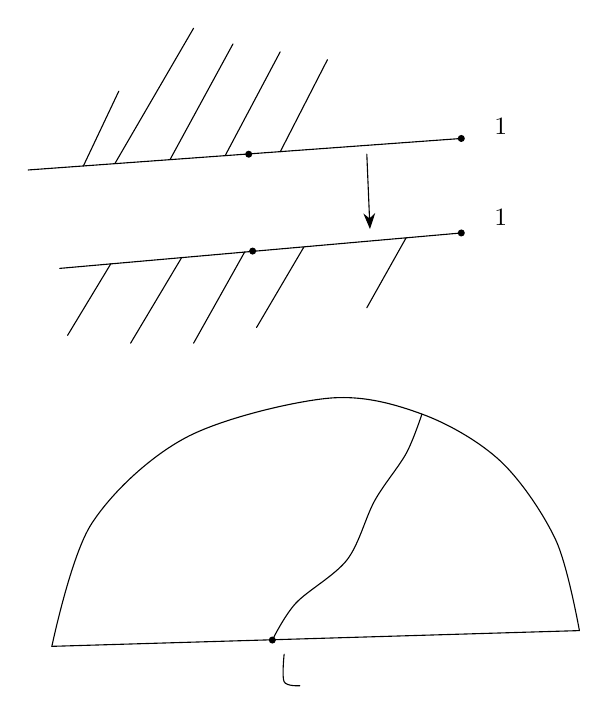
\begin{tikzpicture}[x=1mm,y=1mm,line cap=round,line join=round,font=\scriptsize]
\draw (12,-83) -- (67,-79);
\node[pt] at (40,-81) {};
\node[pt] at (67,-79) {};
\node[inner sep=1pt] at (72,-77.5) {\small $1$};
\draw (16,-95.5) -- (67,-91);
\node[pt] at (40.5,-93.3) {};
\node[pt] at (67,-91) {};
\node[inner sep=1pt] at (72,-89) {\small $1$};
\draw[-{Stealth[length=2mm]}] (55,-81) -- (55.4,-90.5);
\draw (19,-82.5) -- (23.5,-73);
\draw (23,-82.2) -- (33,-65);
\draw (30,-81.7) -- (38,-67);
\draw (37,-81.2) -- (44,-68);
\draw (44,-80.7) -- (50,-69);
\draw (22.5,-94.9) -- (17,-104);
\draw (31.5,-94.1) -- (25,-105);
\draw (39.5,-93.4) -- (33,-105);
\draw (47,-92.8) -- (41,-103);
\draw (60,-91.6) -- (55,-100.5);
\draw (15,-143.5) -- (82,-141.5);
\draw plot[smooth, tension=0.55] coordinates {(15,-143.5) (20,-128) (32,-117) (50,-112) (62,-114) (72,-120) (79,-130) (82,-141.5)};
\node[pt] at (43,-142.7) {};
\draw plot[smooth, tension=0.55] coordinates {(43,-142.7) (46,-138) (52.5,-132.5) (56,-125) (60,-119) (62,-114)};
\draw plot[smooth, tension=0.55] coordinates {(44.5,-144.5) (44.5,-148) (46.5,-148.5)};
\end{tikzpicture}
\end{document}
